%! Author = noone
%! Date = 8/10/22

% Preamble
\documentclass[11pt]{article}
\documentclass{beamer}

% Packages
\usepackage{amsmath}
\usepackage{graphicx}
\usepackage{float}
\usepackage{multimedia}
\usepackage{blindtext}
\usepackage{hyperref}

% Document
\begin{document}

\section{Statistics of Language}\label{sec:statistics-of-language}
\subsection{Definitions, synonyms and antonyms}\label{subsec:definitions-synonyms-and-antonyms}

How do we capture the true meaning of a word, or its relationship to other words?

Words are sometimes arranged into a taxonomy $-$ for example, a bird is a mammal is an animal, etc.

We can also look at dictionary definitions, or lists of synonyms and antonyms.

Here is a list of synonyms for the word \('\)elegant\('\):

    stylish, graceful, tasteful, discerning, refined, sophisticated, dignified, cultivated, distinguished, classic, smart, fashionable, modish, decorous, beautiful, artistic, aesthetic, lovely; charming, polished, suave, urbane, cultured, dashing, debonair; luxurious, sumptuous, opulent, grand, plush, high-class, exquisite

Human effort is required to compile taxonomies, dictionary definitions and lists of synonyms and antonyms.
Some important relationships may be missing, nuances may be lost.
Words like \('\)king\('\) and \('\)queen\('\) are not quite synonyms nor antonyms because they are similar in some attributes but opposite in others.

Is it possible to extract statistical properties and relationships between words automatically, without human involvement?

We will discuss a number of techniques for statistical language processing, using this children's rhyme as an example.

There was a Crooked Man who walked a crooked mile and found a crooked sixpence upon a crooked stile.
He bought a crooked cat, who caught a crooked mouse, and they all lived together in a little crooked house.

\begin{figure}[H]
    \centering
    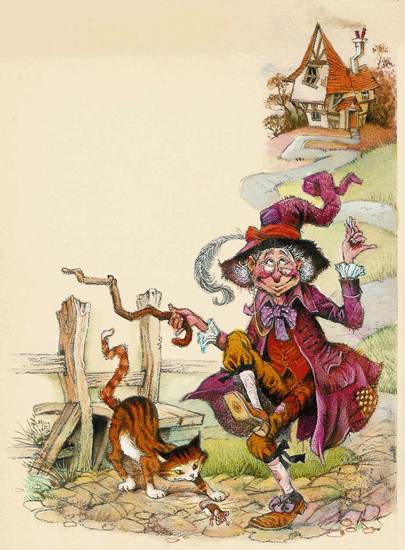
\includegraphics{../out/images/john_patience}
    \caption[john patience]{john patience}
    \label{fig:john patience}
\end{figure}

\section{Singular Value Composition}\label{sec:singular-value-composition}
\subsection{Counting word frequencies}\label{subsec:counting-word-frequencies}
Perhaps the simplest thing we can do to analyse a text is just to count the frequency with which each word occurs.

\begin{figure}[H]
    \centering
    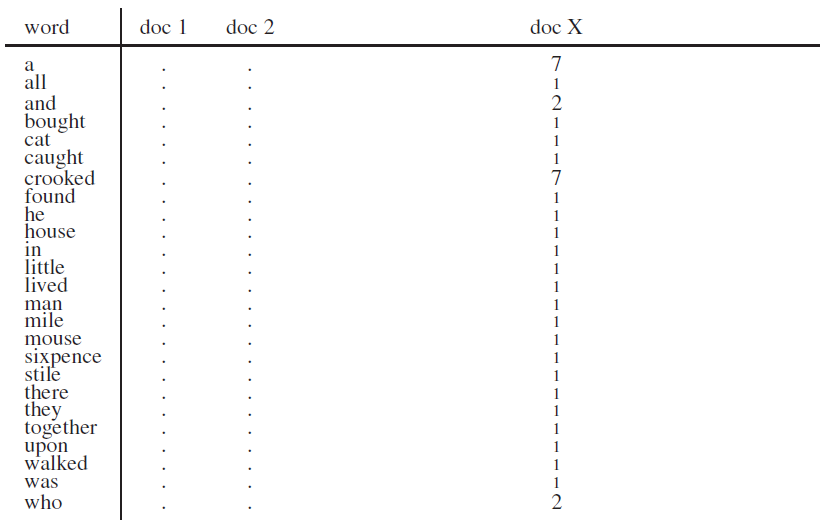
\includegraphics{../out/images/word-count}
    \caption[word count]{word count}
    \label{fig:word count}
\end{figure}

This can be useful for document classification.
Each column of the matrix becomes a vector representing the corresponding document.
Some words like \('\)a\('\), \('\)and\('\) occur frequently in all (or most) documents;
other words occur frequently only in certain types of documents, so are more distinctive.
For example, words like \('\)cat\('\), \('\)mouse\('\), \('\)house\('\) tend to occur in children’s books or rhymes, while other groups of words might be characteristic of legal documents, political news, sporting results, etc.

Words occurring many times in one document may skew the vector.
Sometimes it is better if the matrix entries are just \('1'\) or \('0'\) indicating whether the word occurs at all.

\subsection{counting consecutive words}\label{subsec:counting-consecutive-words}
Another thing we can do is to count the frequency of two words occurring consecutively.

\begin{figure}[H]
    \centering
    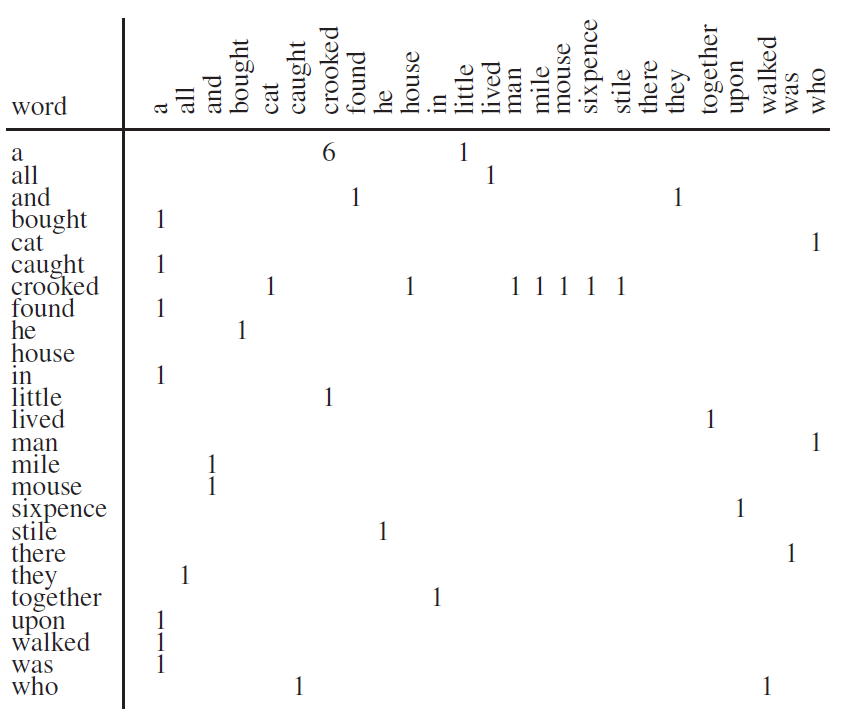
\includegraphics{../out/images/counting-consecutive-words}
    \caption[counting consecutive words]{counting consecutive words}
    \label{fig:counting consecutive words}
\end{figure}

\subsection{Predictive $n$-Gram Word Model}\label{subsec:predictive-$n$-gram-word-model}
If we normalise so that the sum of the entries in each row is equal to $1$, we can use this matrix to estimate the probability $prob(w_j | w_i)$ of word $w_j$ occurring after $w_i$

\begin{figure}[H]
    \centering
    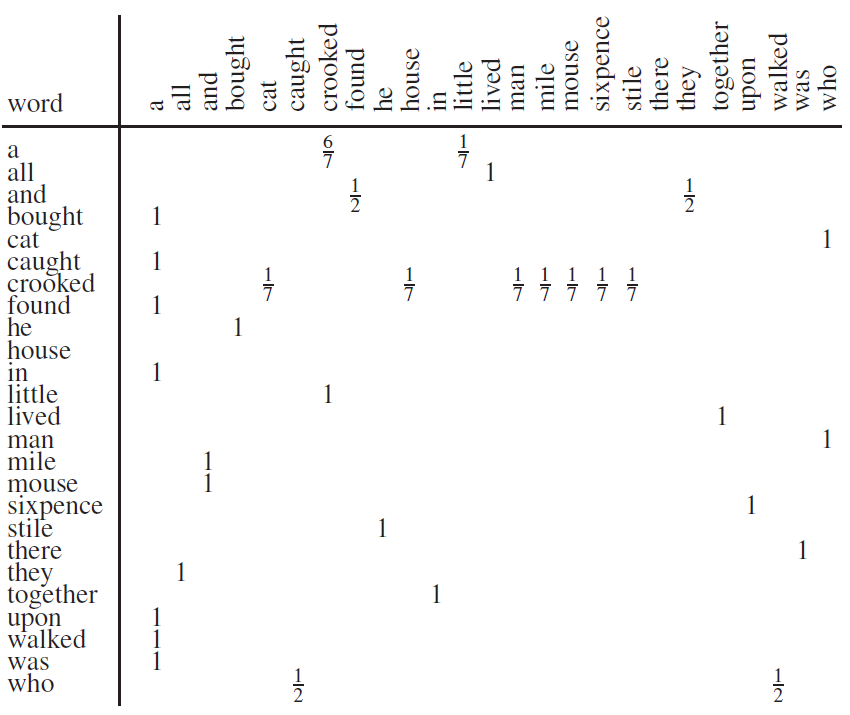
\includegraphics{../out/images/predictive-n-gram-word-model}
    \caption[predictive n-gram word model]{predictive n-gram word model}
    \label{fig:predictive n-gram word model}
\end{figure}

In practice, we need to aggregate over a large corpus, so that unusual words like \("\)crooked\("\) will not dominate.

The above model captures some common combinations like “there was”, “man who”, “and found”, “he bought”, “who caught”, “and they”, “they all”, “lived together”, etc.

This unigram model can be generalised to a bi-gram, tri-gram, . . . , nnn-gram model by considering the nnn preceding words.
If the vocabulary is large, we need some tricks to avoid exponential use of memory.

\subsection{Unigram Text Generator}\label{subsec:unigram-text-generator}
Here is an example of text generated from a unigram model based on the frequencies of word pairs in Shakespeare's Hamlet.

“Rashly – Good night is very liberal – it is easily said there is – gyved to a sore distraction in wrath and with my king may choose but none of shapes and editing by this, and shows a sea And what this is miching malhecho;
And gins to me a pass, Transports his wit, Hamlet, my arms against the mind impatient, by the conditions that would fain know;
which, the wicked deed to get from a deed to your tutor.”

We see that the local structure looks plausible, but the global structure seems like gibberish.

\subsection{Co-occurrence Matrix}\label{subsec:co-occurrence-matrix}
Sometimes, we don’t necessarily predict the next word, but simply a “nearby word” (e.g.\ a word occurring within an $n$-word window centered on that word).

For this case, we can build a matrix in which each row represents a word, and each column a nearby word.
Co-occurrence Matrix (2-word window)

\subsection{Co-occurrence Matrix (10-word window)}\label{subsec:co-occurrence-matrix-(10-word-window)}
\begin{figure}[H]
    \centering
    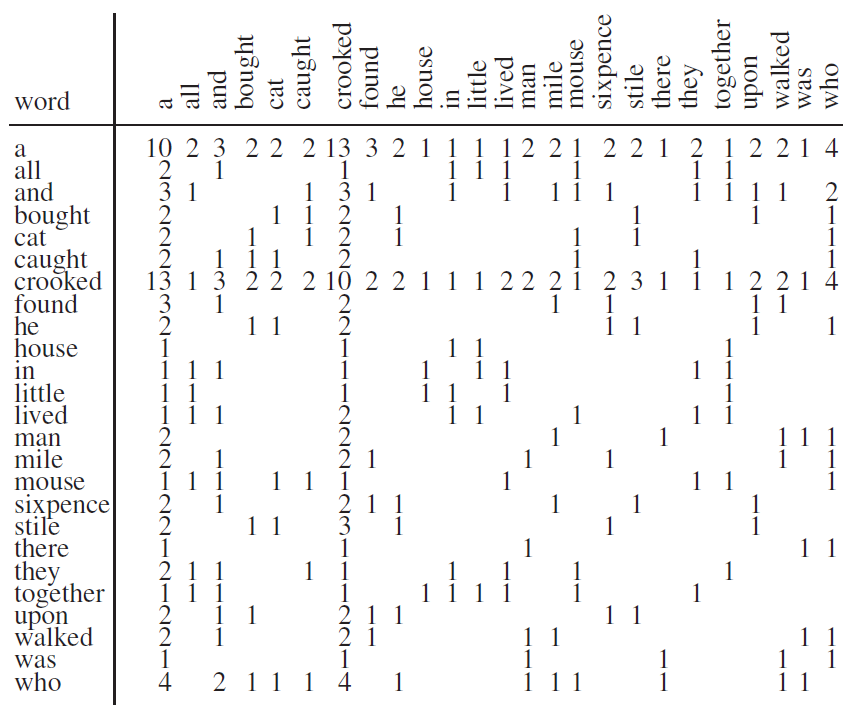
\includegraphics{../out/images/co-occurence-matrix}
    \caption[co-occurence matrix]{co-occurence matrix}
    \label{fig:co-occurence matrix}
\end{figure}
By aggregating over many documents, pairs (or groups) of words emerge which tend to occur near each other (but not necessarily consecutively).
For example:
- \('\)cat\('\), \('\)caught\('\), \('\)mouse\('\)
- \('\)walked\('\), \('\)mile\('\)
- \('\)little\('\), \('\)house\('\)

This analysis raises a number of questions:
- Common words tend to dominate the matrix.
Could we sample common words less often, in order to reveal the relationships of less common words?

- Each row of this matrix could be considered as a vector representation for the corresponding word, but the number of dimensions is equal to the size of the vocabulary, which could be very large (∼ 10510^5105).
Is there a way to reduce the dimensionality while still preserving the relationships between words?

\subsection{Optional Video}\label{subsec:optional-video}

\section{Singular Value Decomposition}\label{sec:singular-value-decomposition}
\subsection{Word Vectors}\label{subsec:word-vectors}
\textif{“Words that are used and occur in the same contexts tend to purport similar meanings.”} Z. Harris (1954)
\textif{“You shall know a word by the company it keeps.”} J.R.\ Firth (1957)

We would like to assign a vector to each word or document, in such a way that words with nearby representations are likely to occur in similar contexts (or, similar documents have close vectors).

Each column in the co-occurrence matrix could be considered as a vector representation of a word or document.
However, the number of dimensions in this vector would be very large (equal to the size of the vocabulary, which is typically about 60,000).

Singular Value Decomposition (SVD) is a way of projecting these vectors from 60,000 dimensions to about 200 dimensions, in such a way that the relationship between words (or documents) is preserved.
SVD itself is too computationally expensive, so methods like Word2Vec and Glove are introduced which provide a good approximation to SVD with reasonable computing resources.

\subsection{Singular Value Decomposition}\label{subsec:singular-value-decomposition2}
Let $X$ be a (co-)occurrence matrix where each row represents a word, and each column represents either a word (in which case  or a document (in which case $L$, might not be equal).

This matrix  can be decomposed as where $X = USV^T$ where $U_{(L \times L)}, V_{(M \times M)}$ are unitary (all columns have unit length) and $S_{L \times M}$ is diagonal, with diagonal entries $s_1 \geq s_2 \geq \dots \geq s_M \geq 0$

\begin{figure}[H]
    \centering
    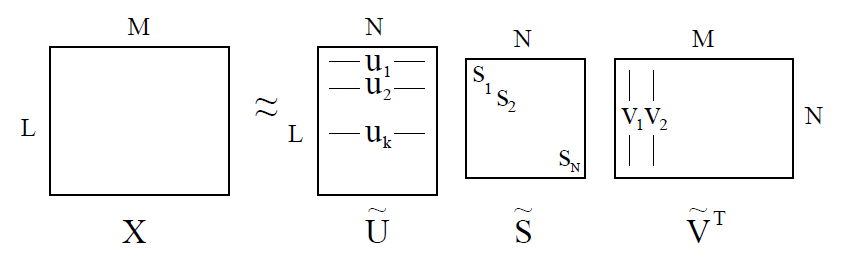
\includegraphics{../out/images/singular-value-decomposition}
    \caption[singular value decomposition]{singular value decomposition}
    \label{fig:singular value decomposition}
\end{figure}

We can obtain an approximation for $X$ of rand $N < M$ by truncating $U$ to $\tilde{U}_{L \times N}$, $S$ to $\tilde{S}_{(N \times N)})$ and $V$ to $\tilde{V}_{(M \times N)}$.
The $k^{th}$ row of $U$ then provides an N-dimensional vector representing the $k^{th}$ word in the vocabulary.
The $k^{th}$ column of $\tilde{V}^T$ also provides an N-dimensional vector, which can be seen either as a representation for documents, or as an alternative representation for words, depending on the origin of the (co-)occurrence matrix.

\subsection{Word2vec and GloVe}\label{subsec:word2vec-and-glove}
Typically, is the number of words in the vocabulary (about 60,000) and $M$ is either equal to $L$ or, in the case of document classification, the number of documents in the collection.
SVD is computationally expensive, proportional to $L \times M^2$ if $L \geq M$

word2vec (Mikolov, 2013) and GloVe (Pennington, 2014) are two common methods for computing an approximation to SVD incrementally, with less computation.
\textbf{word2vec} is a predictive model which aims to maximise the probability of a word, based on the surrounding words.
\textbf{GloVe} is a count-based model which tries to directly reconstruct a close approximation to the co-occurrence matrix $X$.

\subsection{Singular Value compared to Eigenvalue Decomposition}\label{subsec:singular-value-compared-to-eigenvalue-decomposition}
Those familiar with Eigenvalue Decomposition will see that it is similar in some ways to Singular Value Decomposition.
But, we must note a number of important differences, as illustrated in these examples:

Eigenvalue Decomposition
\[\]

Single Value Decomposition
\[\]

\subsection{Singular Value Decomposition}\label{subsec:singular-value-decomposition}:

In general, eigenvalues can be negative or even complex, but singular values are always real and non-negative.
Even if $X$ is a square matrix, singular value decomposition treats the source and target as two entirely different spaces.
The only case where the two decompositions are the same is when $X$ is symmetric and positive semi-definite.
The word co-occurrence matrix is symmetric but not positive semi-definite.
For example, if the text consisted entirely of two alternating letters ..ABABABABABABAB.. then A would be the context for B, and vice-versa.

\subsection{Optional Video}\label{subsec:optional-video2}

\section{Word2Vec}\label{sec:word2vec}
\begin{figure}[H]
    \centering
    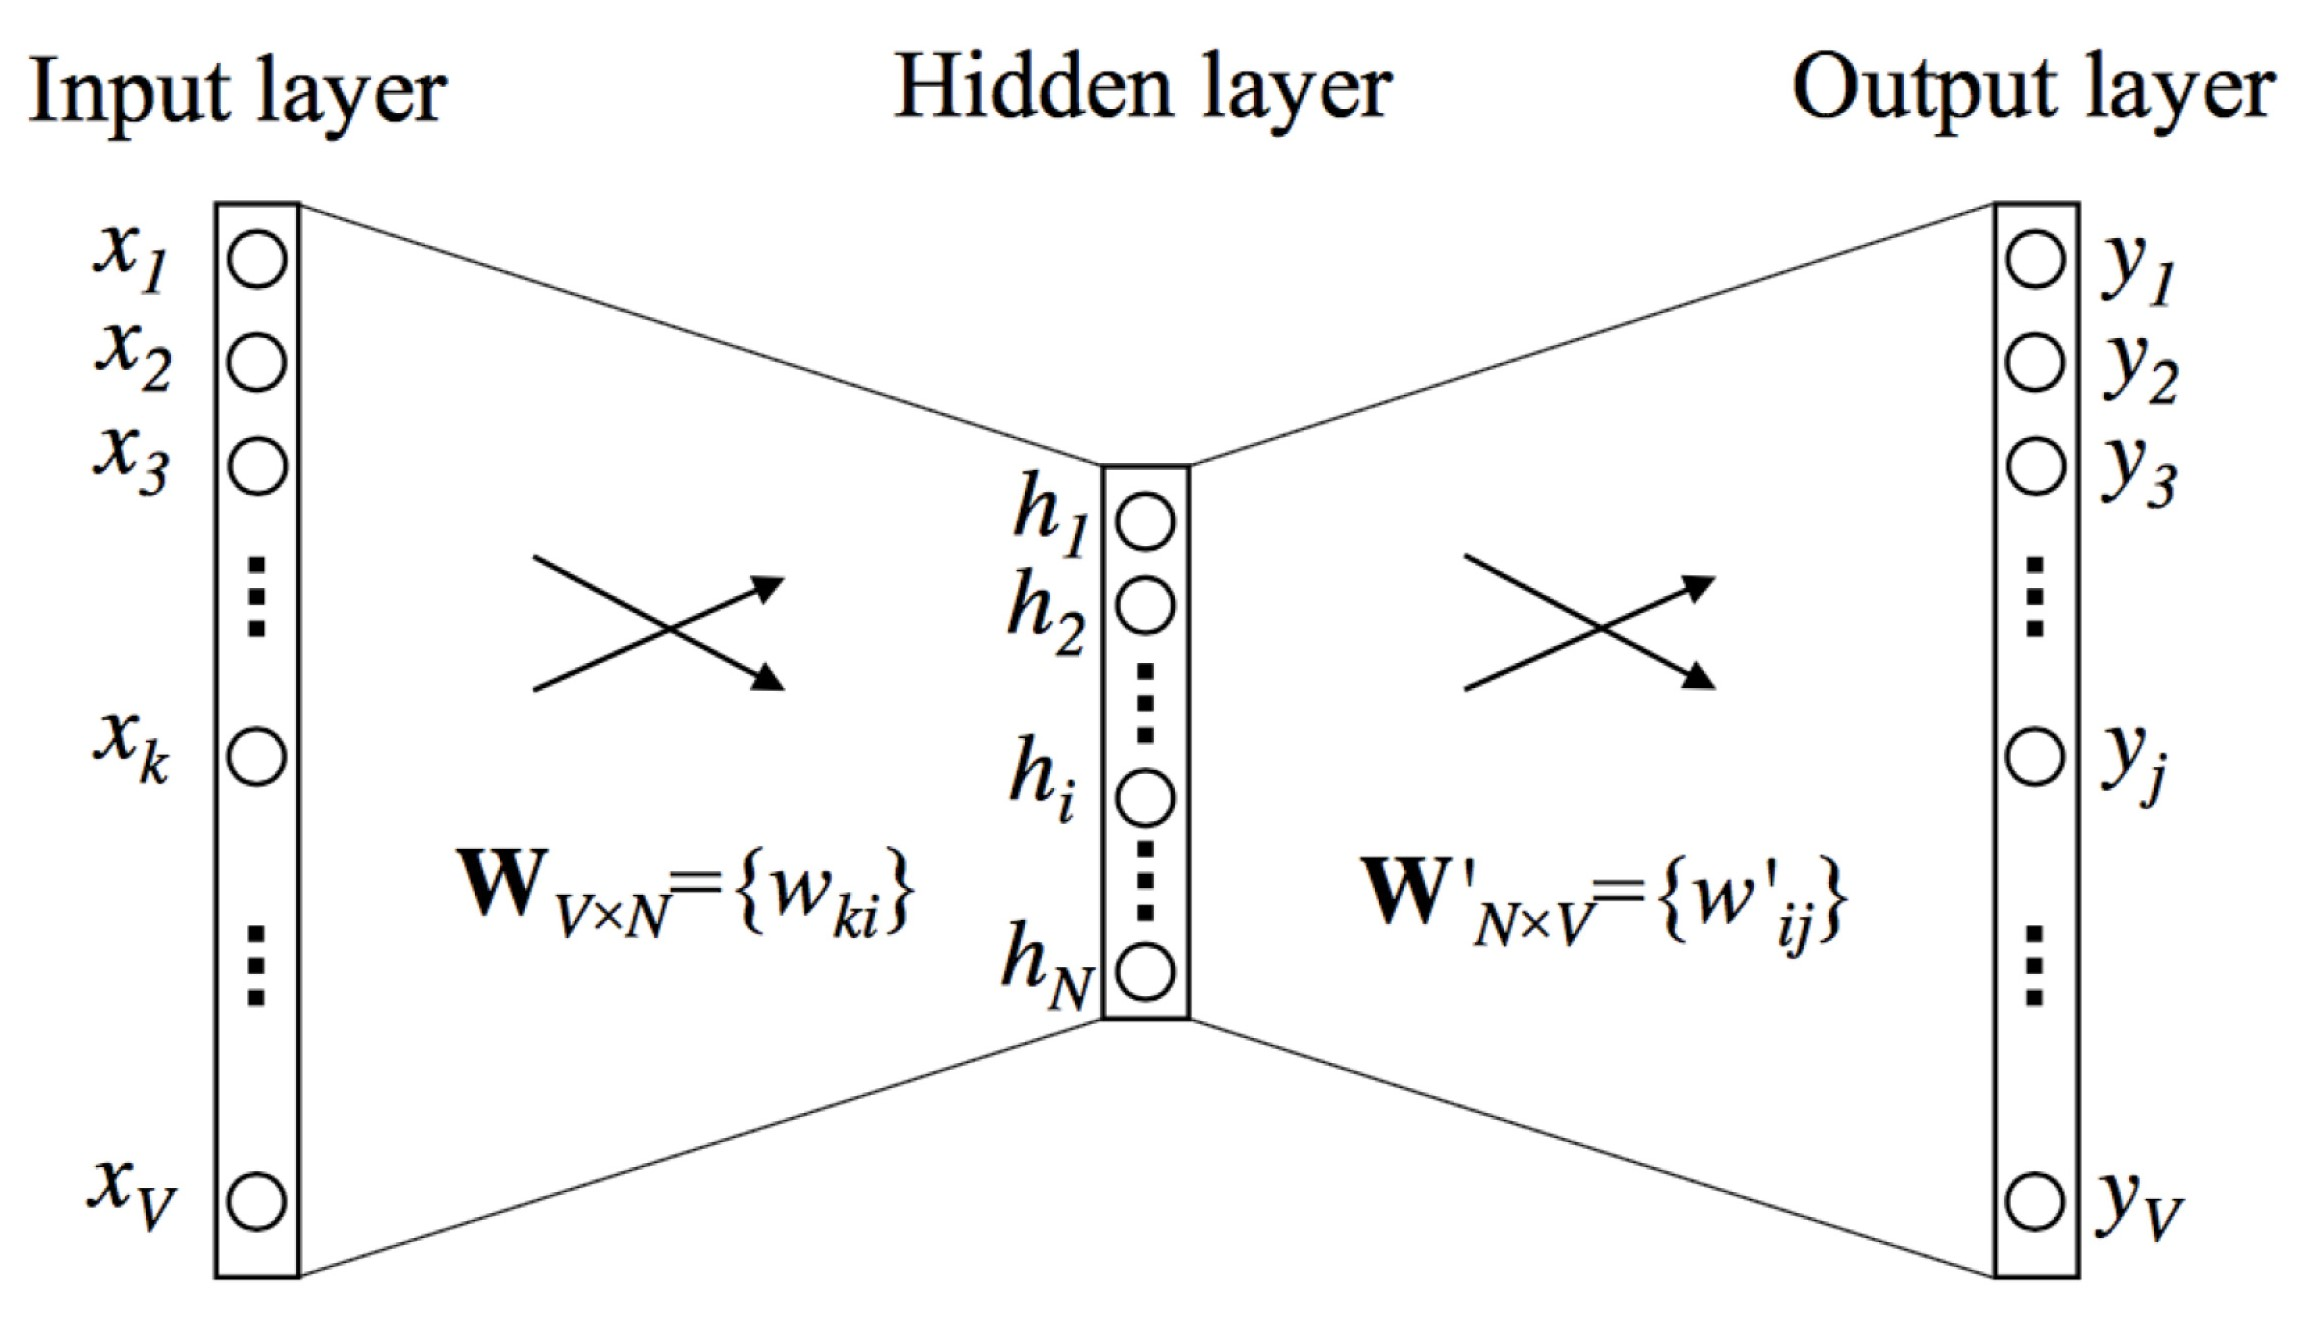
\includegraphics{../out/images/word2vec}
    \caption[word2vec]{word2vec}
    \label{fig:word2vec}
\end{figure}

The $k^{th}$ row $$ of $W$ is a representation of word $k$.

The $$ is an (alternative) representation of word $j$.

If the (1-hot) input is $k$, the linear sum at each output will be

Note that word2vec is a linear model in the sense that there is no activation function at the hidden nodes.

\subsection{Cost function}\label{subsec:cost-function}
Softmax can be used to turn these linear sums  into a probability distribution estimating the probability of word $j$ occurring in the context of word $k$

We can treat the text as a sequence of numbers $a$ means that the $b$ word in the text is the $c$ word in the vocabulary.
We then seek to maximise the log probability

where ccc is the size of training context (which may depend on .

\subsection{word2vec differentials}\label{subsec:word2vec-differentials}
If we assume the probabilities are computed by full softmax, and the correct output is $j\astj^\astj\ast$, then the cost function is

the output differentials are

where

\subsection{word2vec weight updates}\label{subsec:word2vec-weight-updates}

\subsection{hidden-to-output differentials}\label{subsec:hidden-to-output-differentials}

\subsection{hidden unit differentials}\label{subsec:hidden-unit-differentials}

\subsection{input-to-hidden differentials}\label{subsec:input-to-hidden-differentials}

\subsection{Continuous Bag of Words and Skip-Gram}\label{subsec:continuous-bag-of-words-and-skip-gram}
word2vec can be implemented either as Continuous Bag of Words (CBOW) or Skip-Gram, as illustrated in these figures from [Rong, 2014].

\begin{figure}[H]
    \centering
    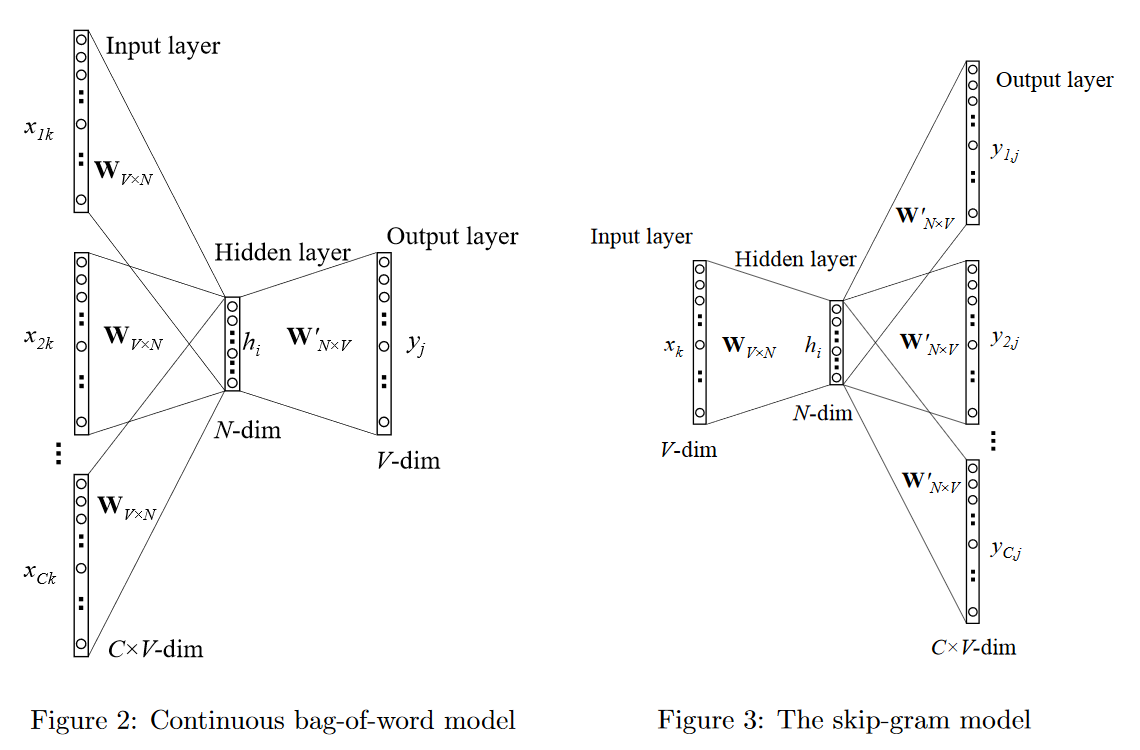
\includegraphics{../out/images/continuous-bag-of-words}
    \caption[continuous bag of words]{continuous bag of words}
    \label{fig:continuous bag of words}
\end{figure}

For CBOW, several context words are each used independently to predict the centre word, and the hidden activation becomes a sum (or average) over all the context words.

Note the difference between this and NetTalk $-$ in word2vec (CBOW) all context words share the same input-to-hidden weights.

The Skip-Gram version tries to predict the context words, given the centre word.
This is similar to CBOW, except that in this case a single input word is used to predict multiple context words, and all context words share the same hidden-to-output weights.

\subsection{Efficiency issues}\label{subsec:efficiency-issues}
Depending on the computational resources available, it may be prohibitively expensive to use the full softmax, which involves computing output values for all 60,000 words in the vocabulary.
Hierarchical Softmax and negative sampling are two alternatives which are computationally more efficient.

\subsection{Hierarchical Softmax}\label{subsec:hierarchical-softmax}
For Hierarchical Softmax, the words are arranged in a Huffmann coded tree according to their frequency.
One network output (with sigmoid activation) is assigned to each node in the tree, and the output corresponding to each node in the path from the root to the actual word is trained to produce either 0 or 1 depending on whether the left or right branch should be taken.
In this way, the total number of outputs is the same, but if the size of the vocabulary is $L$ then only $\log_2(L)$ outputs need to be evaluated, on average, for each word in the training text.

\subsection{Negative sampling}\label{subsec:negative-sampling}
The idea of negative sampling is that we train the network to increase its estimation of the target word j∗j^*j∗ and reduce its estimate not of all the words in the entire vocabulary but instead just a subset of them, drawn from an appropriate distribution.

\[E = -\log \sigma(v'_{j*}^T) - \sum_{j \in W_{neg}} \log \sigma (-v'_{j}^{T}h)\]

This is a simplified version of Noise Contrastive Estimation (NCE).
It is not guaranteed to produce a well-defined probability distribution, but in practice it does produce high-quality word embeddings.

The number of samples is 5--20 for small datasets, 2--5 for large datasets.

Empirically, a good choice of the distribution from which to draw the negative samples is $P(w) = U(w)^{3/4} / Z$ where $U(w)$ is the unigram distribution determined by the previous word, and $Z$ is a normalizing constant.

\subsection{Subsampling of frequent words}\label{subsec:subsampling-of-frequent-words}
In order to diminish the influence of more frequent words, each word in the corpus is discarded with probability

\[P(w_i) = 1 - \sqrt{\dfrac{t}{f(w_i)}}\]

where $f(w_i)$ is the frequency of word $t ~ 10^{-5}$ is an empirically determined threshold.

\subsection{Optional Video}\label{subsec:optional-video3}

\section{Word Relationships}\label{sec:word-relationships}
\subsection{Sentence Completion Task}\label{subsec:sentence-completion-task}

One way to test the quality of the word embeddings is by using them to answer sentence completion tasks from standardised tests such as the Scholastic Aptitude Test (SAT).

\textbf{Q1}
Seeing the pictures of our old home made me feel _______ and nostalgic.

\begin{itemize}
  \item A. fastidious
  \item B. indignant
  \item C. wistful
  \item D. conciliatory
\end{itemize}

This kind of question can be answered by feeding the surrounding words into the CBOW version of the network and seeing which of A,B,C,D{\rm A, B, C, D}A,B,C,D is assigned the highest probability by the network.

\textbf{Q2}
Because the House had the votes to override a presidential veto, the President has no choice but to ____________ .

\begin{itemize}
  \item A. object
  \item B. abdicate
  \item C. abstain
  \item D. compromise
\end{itemize}

The network might have some difficulty answering questions like Q2, because of the need for logical reasoning or culturally specific knowledge.

\section{Word Relationships}\label{sec:word-relationships2}
Another way to probe the word vectors is to look for linguistic regularities.
For example, if we add the vectors for $\text{King}$ and $\text{Woman}$ and subtract the vector for $\text{Man}$, we get something very close to the vector for $\text{Queen}$, i.e.

\[\text{King} + \text{Woman} - \text{Man} \simeq \text{Queen}\]

This can be used to answer questions of the form: $A$ is to $B$ as $B$ is to What?
For example:

\textbf{Q3}
evening is to morning as dinner is to _______ .
\begin{itemize}
  \item A. breakfast
  \item B. soup
  \item C. coffee
  \item D. time
\end{itemize}

\text{Q4}
bow is to arrow as ______ is to bullet.

\begin{itemize}
  \item A. defend
  \item B. lead
  \item C. shoot
  \item D. gun
\end{itemize}

In each case, we look for the word $X$ in the dictionary whose vector is closest to $(v_C + v_B - v_A)$, with closeness determined by cosine similarity.

\[X = \arg \max \dfrac{(v_C + v_B -v_A)^T v_X}{||v_C + v_B -v_A||}\]

Here are some examples of word relationships from (Mikolov, 2013).

\begin{figure}[h]
    \centering
    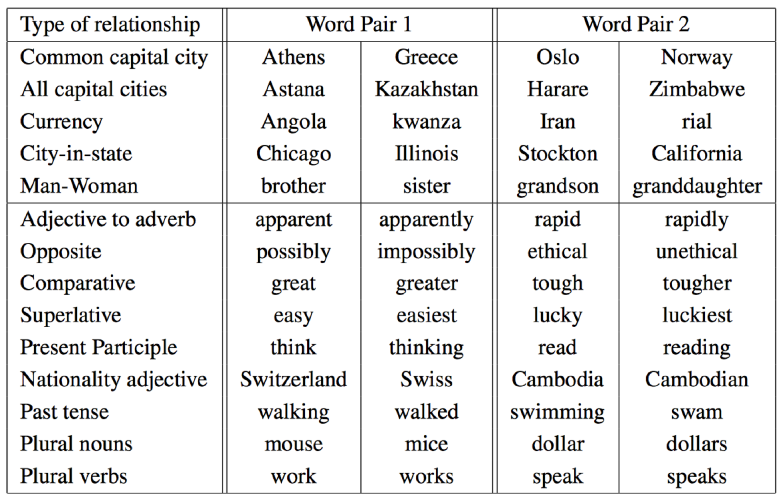
\includegraphics[width=12,height=12]{../out/images/word-relationships}
    \caption[word relationships]{word relationships}
    \label{fig:word relationships}
\end{figure}

\begin{figure}[h]
    \centering
    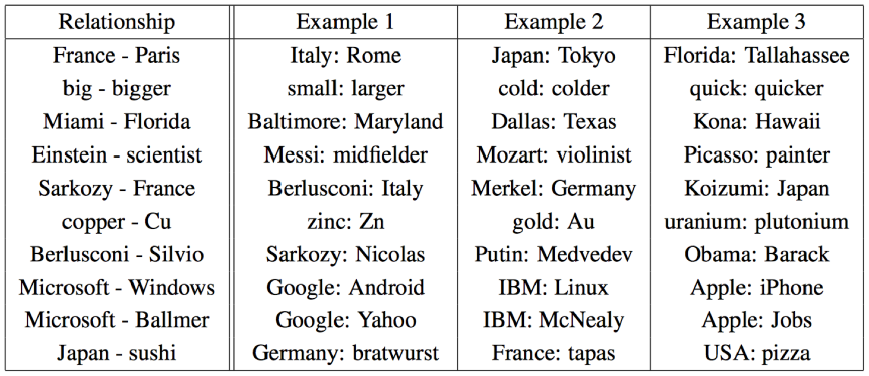
\includegraphics[width=12,height=12]{../out/images/word-relationships-2}
    \caption[word relationships 2]{word relationships 2}
    \label{fig:word relationships 2}
\end{figure}

The network generally performs very well, but occasionally makes an understandable mistake.
For example, did you notice what the network thinks is the first and last name of the President of Russia?

\subsection{Optional Video}\label{subsec:optional-video4}

\section{Exercises}\label{sec:exercises}
Consider the sentence:

\textif{"two flowers grew tall on two tall towers"}

\textbf{Question 1}

Write the co-occurrence matrix $X$ for this sentence, using a 4-word context window (i.e. two context words on either side of the central word).

\textbf{Answer}

\textbf{Question 2}
Use `torch.svd()` to compute the singular value decomposition of this matrix $X = UST^T$.

\textbf{Answer}

\textbf{Question 3}
Extract a word representation from the first two columns of $U$ and use matplotlib to plot the words on a 2-dimensional graph.

\textbf{Answer}

\end{document}